\documentclass[titlepage]{article}
%Compile with pdflatex%
\title{CS 1632 -- DELIVERABLE 4\\
PROPERTY-BASED TESTING\\
\small{\url{https://github.com/blester125/CS_1632_deliverable4}}}
\author{Brian Lester}
\usepackage{hyperref}
\usepackage{graphicx}
\usepackage{listings}
\begin{document}
\maketitle
\section{Summary}
For deliverable 4 I choose to do property based testing of Java's built in 
sorting function \lstinline!Arrays.sort(int[] arr)!. I chose this project over 
the combinatorial testings because the idea of property based testing was 
appealing to me. The fact that this kind of testing grew out of functional 
programming is especially interesting to me as I am currently learning Haskell. 

To start I began by writing the code that generates that random arrays. This was 
rather simple. The next thing I figured out was the properties that I wanted to 
test. The first one that I wanted to test was obvious the output should be 
sorted, otherwise what good would the sorting method be? This is easy to test 
because you just have to check if each value is less than or equal to the one 
after it. The other properties are ones we discussed in class. That the size of 
output is equal to the size of the input, that the sort function is pure (that is 
two equal inputs produces the same output), and that it is idempotent (running 
the function on the output of the function doesn't change the output). These were 
all discussed in class or in the book.

Writing the test themselves are rather easy. The closest thing I had to a problem 
was when I needed to duplicate the arrays. I knew that I couldn't simple say \
\lstinline!int[] newArray = oldArray! because this would make a shallow copy so I 
wrote a function that copied the contents of one array into new array. Just as I 
finished this function I rememberer that I could create a deep copy of the array 
using the \lstinline{.clone()} method. The code can be found at: \\
\url{https://github.com/blester125/CS_1632_deliverable4}

This form of testing is really cool and seems really powerful. The downside is 
that this form seems like it would be difficult to test certain functions. I plan 
to continue to use this form of testing and to investigate the quick check 
libraries that are more in-line with this form of testing.

\section{JUnit Tests Screenshot}
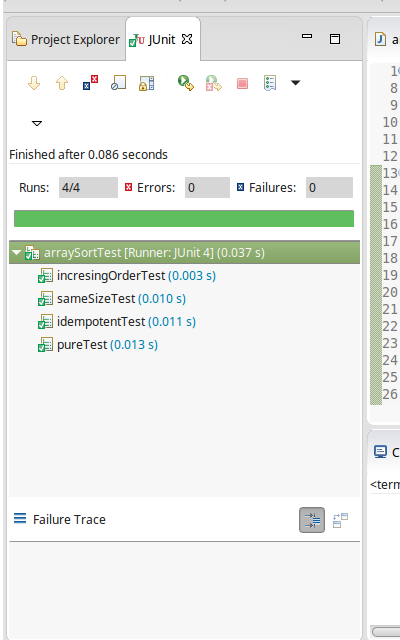
\includegraphics[width=.75\textwidth,natwidth=400,natheight=640]{PropertyBasedTest.png}
\end{document}